
\chapter{Introduction}
\raggedbottom

Marine phytoplankton are central players in the global carbon cycle, responsible for nearly half of global primary production. The identification of the major factors controlling phyto- plankton ecology, physiology, and, ultimately, bloom dynamics has been a central problem in the field of biological oceanography for the past century. From physical explanations (Sverdrup’s critical depth hypothesis), to chemical rational (Redfield ratio), to ecological theory (Margalef’s mandala), the field has been constantly reevaluating evidence to answer the question: What drives phytoplankton blooms? Molecular approaches enable the di- rect examination of species-specific metabolic profiles in mixed, natural communities, a task which was previously intractable. In this thesis, I developed and applied novel analytical tools and bioinformatic pipelines to characterize the physiological response of phytoplank- ton at various levels of taxonomic grouping (strain, species, and functional group) to their environment.

A diverse community of marine microorganisms are at the heart of the global carbon cycle, creating and transforming dissolved organic matter, 


Photosynthesis by marine phytoplankton (small floating photosynthetic organisms) represents nearly 50\% of the total primary production on earth (1). Climate change is predicted to alter the biogeochemistry of the world's oceans (2) as well as the distribution and nature of primary production in the global surface ocean (3). Despite being of central importance, fundamental uncertainties remain regarding the basic ecology and biology of phytoplankton, such as: 1) How do phytoplankton respond to changing (light, nutrient, temperature) environments? 2) What enables the maintenance of diverse phytoplankton communities? 3) How does community structure influence ecosystem function and biogeochemical cycling? 
As with the field of medicine, advances in sequencing and mass spectrometry over the last decade have accelerated the field of biological oceanography. The burgeoning technologies fueling the ``-omics''\footnote{``-omics'' is a catch-all suffix typically used to describe large, molecular datasets (e.g. genomics, the study of the genome, and transcriptomics, the study of the complete set of RNA transcripts produced under certain conditions). The use of this suffix, however, is expanding to other fields (see \href{https://twitter.com/search?q=\%23badomics&src=typd&lang=en}{\#badomics}). }  revolution allow a unique glimpse at the previously hidden molecular world of the microbes, enabling the tracking of species-specific metabolism in the environment. Capitalizing upon this revolution to address biogeochemical or ecological questions, however, is becoming increasingly difficult, as our ability to make measurements has surpassed our ability to analyze, visualize, and compare the data produced. My background and training in oceanography, microbiology, bioinformatics, and art make me uniquely poised to work on these informatics problems. During my PhD, I developed pipelines (4, 5) and bioinformatic tools (6) for the analysis of meta -transcriptomic datasets to interrogate the ecology and biogeochemical function of microbes in marine systems. With the University of California Postdoctoral Presidential Fellowship, I would be able to expand upon my existing computation skill set by integrating with the Lab for Data Intensive Biology headed by C. Titus Brown at UC Davis. Dr. Brown’s lab works to develop tools and approaches to extract meaningful information from large, unwieldy datasets. My research goal is to integrate multiple environmental and “meta-omic” datasets to examine the species-specific physical and chemical drivers of phytoplankton bloom formation. 


%\section

%Microorganisms are the numerically 


%Appreciate for the 
%Over the past two decades technological advances from the medical field have migrated to the field of biological oceanography. 

%Despite the impressive advances that have been made in assessing the diversity of marine microorganisms, the mechanisms that underlie the participation of microorganisms in marine food webs and biogeochemical cycles are poorly understood. Here, we stress the need to examine the biochemical interactions of microorganisms with ocean systems at the nanometre to millimetre scale — a scale that is relevant to microbial activities. The local impact of microorganisms on biogeochemical cycles must then be scaled up to make useful predictions of how marine ecosystems in the whole ocean might respond to global change. This approach to microbial oceanography is not only helpful, but is in fact indispensable.
%\section{}

%\section{}

%\section{}

%Photosynthetic microbes dominate the primary production of the ocean and account for roughly half of all primary production on earth [Field]; The diversity 
%Chapter two describes the architecture of the $\mu$FPU unit, and the
%motivations for the design decisions made.


\begin{figure}[h!]
  \centering
    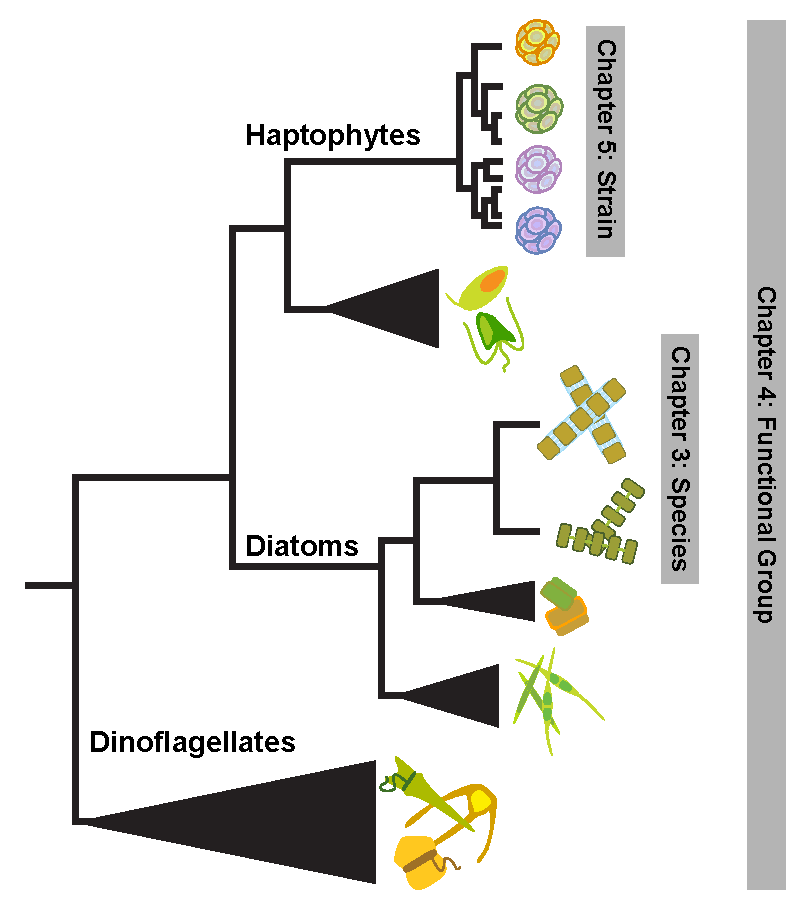
\includegraphics[width=.7\textwidth]{Images/C1_ThesisDiagram.pdf}
    \caption{Conceptual overview of the levels of diversity explored in chapters 3, 4, and 5 of this thesis.}
  \label{fig:c1f1}
\end{figure}



